\documentclass[11pt]{article}
\usepackage[margin=0.5cm,papersize={24cm,12cm}]{geometry}
\usepackage[utf8]{inputenc}
\usepackage[T1]{fontenc}
\usepackage{amsmath,amssymb}
\usepackage{xcolor}
\usepackage{tikz}
\usetikzlibrary{positioning,calc,arrows.meta}
\pagestyle{empty}

\definecolor{Ink}{HTML}{1F2D3D}
\definecolor{Muted}{HTML}{667085}
\definecolor{Grid}{HTML}{E8ECF3}

\definecolor{Stat}{HTML}{4E79A7}
\definecolor{Seq}{HTML}{59A14F}
\definecolor{GAN}{HTML}{F28E2B}
\definecolor{Diff}{HTML}{6B5FDB}
\definecolor{FM}{HTML}{C65C95}

\definecolor{BandBlue}{HTML}{EDF3FB}
\definecolor{BandGreen}{HTML}{EDF7EF}
\definecolor{BandOrange}{HTML}{FFF0E1}
\definecolor{BandPurple}{HTML}{F1EEFF}
\definecolor{BandPink}{HTML}{FCEBF4}

\newcommand{\MethodBoxClean}[4][2.15cm]{%
\node[rounded corners=2pt, draw=#2!65!black, fill=white, line width=0.45pt,
      minimum width=#1, minimum height=1.15cm, align=center,
      inner sep=1.5pt, text=Ink] at #3 {%
  \begin{tabular}{@{}c@{}}
    {\scriptsize\bfseries #4}
  \end{tabular}%
};
}

\newcommand{\FamilyBlockClean}[7][4.95cm]{%
\node[rounded corners=6pt, draw=#2!70!black, fill=#3,
      minimum width=#1, minimum height=4.00cm, inner sep=0pt] (#4) at #5 {};
\node[anchor=north west, font=\bfseries\small, text=Ink]
at ([xshift=4mm,yshift=-1.5mm]#4.north west) {#6};
\draw[#2!55!black, line width=0.55pt]
([xshift=3mm,yshift=-8mm]#4.north west) -- ([xshift=-3mm,yshift=-8mm]#4.north east);
#7
}

\begin{document}
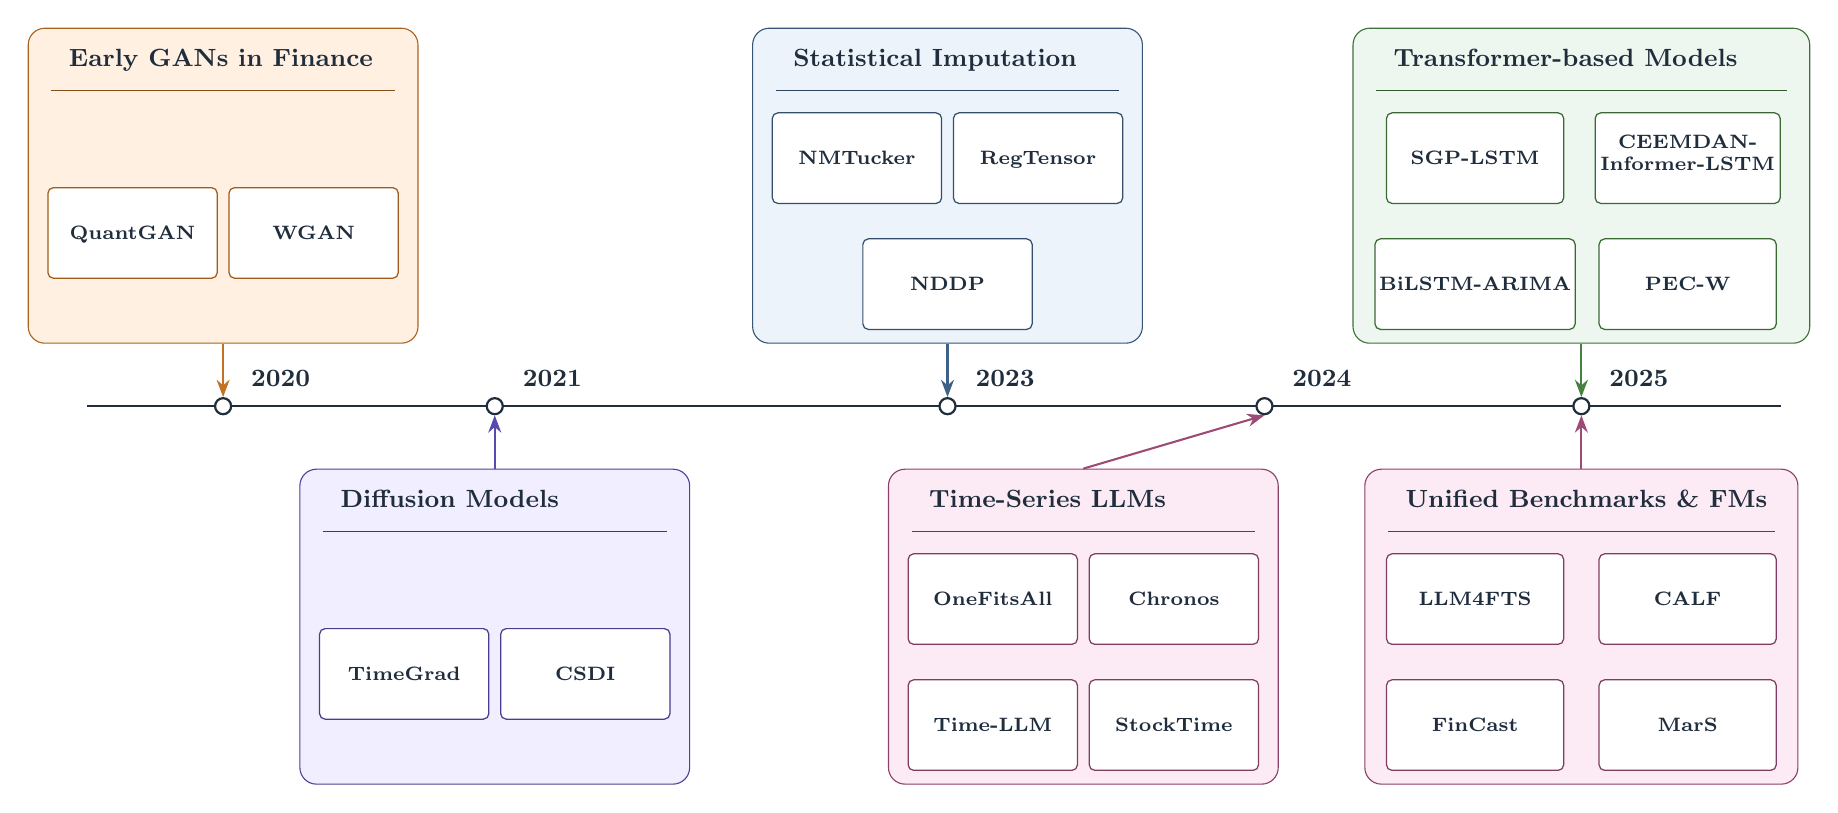
\begin{tikzpicture}[
    x=1.15cm,
    y=1cm,
    every node/.style={font=\normalsize}
]

% Timeline
\draw[thick, Ink] (-1.5, 0) -- (17.2, 0);

\foreach \year/\x in {2020/0, 2021/3.0, 2023/8.0, 2024/11.5, 2025/15.0} {
    \node[circle, draw=Ink, thick, fill=white, minimum size=5.8pt, inner sep=0pt] (y\year) at (\x,0) {};
}

\node[above right=0.5mm and 1.5mm of y2020, font=\bfseries\small, text=Ink] {2020};
\node[above right=0.5mm and 1.5mm of y2021, font=\bfseries\small, text=Ink] {2021};
\node[above right=0.5mm and 1.5mm of y2023, font=\bfseries\small, text=Ink] {2023};
\node[above right=0.5mm and 1.5mm of y2024, font=\bfseries\small, text=Ink] {2024};
\node[above right=0.5mm and 1.5mm of y2025, font=\bfseries\small, text=Ink] {2025};

% GAN -> 2020
\FamilyBlockClean{GAN}{BandOrange}{nGAN}{(0,2.8)}{Early GANs in Finance}{
  \MethodBoxClean{GAN}{([xshift=-11.5mm,yshift=-6mm]nGAN.center)}{QuantGAN}
  \MethodBoxClean{GAN}{([xshift=11.5mm,yshift=-6mm]nGAN.center)}{WGAN}
}{}
\draw[-{Stealth[length=2.2mm]}, GAN!80!black, line width=0.75pt]
(nGAN.south) -- (y2020.north);

% Statistical Imputation -> 2023
\FamilyBlockClean{Stat}{BandBlue}{nImp}{(8.0,2.8)}{Statistical Imputation}{
    \MethodBoxClean{Stat}{([xshift=-11.5mm,yshift=3.5mm]nImp.center)}{NMTucker}
    \MethodBoxClean{Stat}{([xshift=11.5mm,yshift=3.5mm]nImp.center)}{RegTensor}
    \MethodBoxClean{Stat}{([xshift=0mm,yshift=-12.5mm]nImp.center)}{NDDP}
}{}
\draw[-{Stealth[length=2.2mm]}, Stat!80!black, line width=0.75pt]
(nImp.south) -- (y2023.north);

% Transformer-based Models -> 2025 (Wider box: 5.8cm to eliminate overflow)
\FamilyBlockClean[5.8cm]{Seq}{BandGreen}{nTrans}{(15.0,2.8)}{Transformer-based Models}{
    \MethodBoxClean[2.25cm]{Seq}{([xshift=-13.5mm,yshift=3.5mm]nTrans.center)}{SGP-LSTM}
    \MethodBoxClean[2.35cm]{Seq}{([xshift=13.5mm,yshift=3.5mm]nTrans.center)}{\shortstack{CEEMDAN-\\Informer-LSTM}}
    \MethodBoxClean[2.25cm]{Seq}{([xshift=-13.5mm,yshift=-12.5mm]nTrans.center)}{BiLSTM-ARIMA}
    \MethodBoxClean[2.25cm]{Seq}{([xshift=13.5mm,yshift=-12.5mm]nTrans.center)}{PEC-W}
}{}
\draw[-{Stealth[length=2.2mm]}, Seq!80!black, line width=0.75pt]
(nTrans.south) -- (y2025.north);

% Diffusion Models -> 2021
\FamilyBlockClean{Diff}{BandPurple}{nDiff}{(3.0,-2.8)}{Diffusion Models}{
  \MethodBoxClean{Diff}{([xshift=-11.5mm,yshift=-6mm]nDiff.center)}{TimeGrad}
  \MethodBoxClean{Diff}{([xshift=11.5mm,yshift=-6mm]nDiff.center)}{CSDI}
}{}
\draw[-{Stealth[length=2.2mm]}, Diff!80!black, line width=0.75pt]
(nDiff.north) -- (y2021.south);

% Time-Series LLMs -> 2024
\FamilyBlockClean{FM}{BandPink}{nLLM}{(9.5,-2.8)}{Time-Series LLMs}{
    \MethodBoxClean{FM}{([xshift=-11.5mm,yshift=3.5mm]nLLM.center)}{OneFitsAll}
    \MethodBoxClean{FM}{([xshift=11.5mm,yshift=3.5mm]nLLM.center)}{Chronos}
    \MethodBoxClean{FM}{([xshift=-11.5mm,yshift=-12.5mm]nLLM.center)}{Time-LLM}
    \MethodBoxClean{FM}{([xshift=11.5mm,yshift=-12.5mm]nLLM.center)}{StockTime}
}{}
\draw[-{Stealth[length=2.2mm]}, FM!80!black, line width=0.75pt]
(nLLM.north) -- (y2024.south);

% Unified Benchmarks & FMs -> 2025
\FamilyBlockClean[5.5cm]{FM}{BandPink}{nUni}{(15.0,-2.8)}{Unified Benchmarks \& FMs}{
    \MethodBoxClean[2.25cm]{FM}{([xshift=-13.5mm,yshift=3.5mm]nUni.center)}{LLM4FTS}
    \MethodBoxClean[2.25cm]{FM}{([xshift=13.5mm,yshift=3.5mm]nUni.center)}{CALF}
    \MethodBoxClean[2.25cm]{FM}{([xshift=-13.5mm,yshift=-12.5mm]nUni.center)}{FinCast}
    \MethodBoxClean[2.25cm]{FM}{([xshift=13.5mm,yshift=-12.5mm]nUni.center)}{MarS}
}{}
\draw[-{Stealth[length=2.2mm]}, FM!80!black, line width=0.75pt]
(nUni.north) -- (y2025.south);

\end{tikzpicture}
\end{document}
